\section{Training-Time Policy Optimization}
\label{sec:training}

Section 4 tests whether sequence-level fine-tuning can improve a near-converged CTC model — §3's result that CTC backward implements a Rao-Blackwellized REINFORCE estimator makes the question precise, and neither experiment produces improvement. The failures are diagnostic: two mechanisms distinguishable under the tested configurations that together define where sequence-level fine-tuning at near-converged CTC checkpoints breaks down.



\subsection{Experimental Setup}

\subsubsection{Model and data}

The primary model for §4.2 is the Zipformer-S CR-CTC checkpoint \cite{yao2024zipformer, huang2024crctc} released via the icefall recipe library \cite{li2022k2}. It has 22.1M parameters and uses a BPE-500 vocabulary. Training used the LibriSpeech train-clean-100 subset \cite{panayotov2015librispeech} (100 hours of clean read speech), with evaluation on dev-other ($n = 2864$ utterances) and dev-clean ($n = 2703$ utterances). We used corpus-level WER throughout: total edit distance divided by total reference word count, matching the standard LibriSpeech evaluation protocol \cite{panayotov2015librispeech}.

\subsubsection{N-best generation}

We generated candidate sets by sampling from k2 CTC lattices at \texttt{nbest\_scale=1.0} with 4$\times$ oversampling followed by deduplication. We used $G = 4$ candidates per utterance during training and $G = 16$ for evaluation, following the MWER setup of \citet{prabhavalkar2018mwer}. The canonical value \texttt{nbest\_scale=1.0} is mandatory: setting it to 0.5 destroys approximately 90% of the oracle gap by sharpening the lattice beyond the diversity needed for reward signal (see Appendix~B.2 for quantitative scale-sensitivity results).

\subsubsection{Four MWER configurations}

We trained four configurations of MWER on the CR-CTC model:

- \textbf{MWER-unclipped-subset}: standard MWER (no gradient clipping), lr$=10^{-5}$, 10 epochs over the first 1000 utterances per epoch.
- \textbf{MWER-clipped-subset}: MWER with GRPO-style importance-ratio clipping \cite{shao2024grpo}, same lr and epoch count as MWER-unclipped-subset.
- \textbf{MWER-unclipped-full}: standard MWER at lr$=10^{-5}$, 1 full epoch (7132 steps) over all of train-clean-100.
- \textbf{MWER-clipped-full}: MWER with clipping, 1 full epoch (7133 steps).

\subsubsection{Clipping formula}

The clipped MWER loss replaces $\hat{A}_i \log P_\text{CTC}(y_i|x)$ in Equation~(4) with the PPO-style surrogate:
\begin{equation*}
  \mathcal{L}_\text{clip}(i) = \min\!\bigl(\rho_i\,\hat{A}_i,\;\mathrm{clip}(\rho_i,\,1-\varepsilon_\text{low},\,1+\varepsilon_\text{high})\cdot\hat{A}_i\bigr), \tag{4a}
\end{equation*}
where $\rho_i = \exp\!\bigl((\log P_{\theta}(y_i|x) - \log P_{\theta_\text{ref}}(y_i|x))\,/\,|y_i|\bigr)$ is the length-normalized sequence-level probability ratio between the current and reference policy. The clip bounds differed between the two clipped configurations: MWER-clipped-subset used $(\varepsilon_\text{low}, \varepsilon_\text{high}) = (0.0003, 0.0006)$ (very tight, to limit step size at small G); MWER-clipped-full used $(0.1, 0.2)$ (standard GRPO range). The reference policy $\theta_\text{ref}$ was synchronized with $\theta$ every four gradient-accumulation steps.

All four shared the same training pipeline baseline of $6.67\%$ WER on dev-other.

\subsubsection{Baseline divergence}

The canonical greedy WER on dev-other is $6.02\%$ (used in §§5–6), whereas the training pipeline baseline is $6.67\%$. The difference arises from a mismatch in filterbank computation: the canonical evaluation pipeline uses 80-dimensional fbank features computed by kaldifeat (a Kaldi-compatible feature extraction library \cite{kaldifeat}), whereas the training pipeline uses features computed within the icefall \texttt{zipformer/} recipe, which applies slightly different pre-emphasis and energy flooring. Both pipelines use the same model weights; no correction is applied to the training results because all §4 comparisons use the $6.67\%$ baseline consistently.



\subsection{MWER on CR-CTC: Catastrophic Collapse}

All four MWER configurations degraded dev-other WER. For subset configurations (exp\_A, exp\_B), evaluation at each of the 10 epochs confirmed monotonic increase throughout training. For full-data configurations (exp\_F3, exp\_G2), only the baseline and the final-epoch evaluation were stored — monotonic increase within the epoch is therefore not confirmed, but the endpoint degradation is established. Table~\ref{tab:mwer-endpoint} summarizes the endpoint results.

\begin{table*}[t]
\centering
\caption{MWER training results on Zipformer-S CR-CTC. Baseline dev-other WER = 6.67\% for all runs. $\Delta$ = absolute change in WER at the final evaluation point.}
\label{tab:mwer-endpoint}
\begin{tabular}{lllrr}
\hline
Configuration & Clipping & Epochs/steps & Final WER (\%) & $\Delta$ (pp) \\
\hline
MWER-unclipped-subset & None & 10 epochs & 13.49 & $+$6.82 \\
MWER-clipped-subset & GRPO clipping & 10 epochs & 12.85 & $+$6.18 \\
MWER-unclipped-full & None & 1 epoch / 7132 steps & 15.30 & $+$8.63 \\
MWER-clipped-full & GRPO clipping & 1 epoch / 7133 steps & 15.57 & $+$8.90 \\
\hline
\end{tabular}
\end{table*}

\begin{figure*}[t]
  \centering
  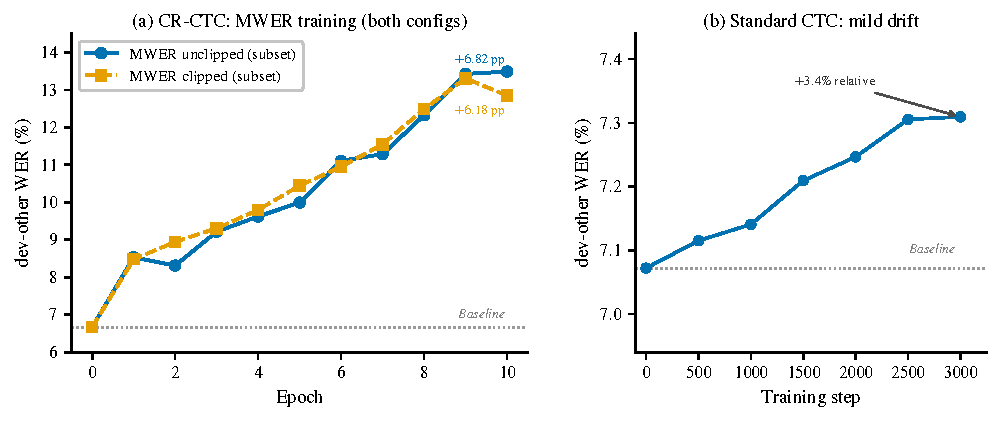
\includegraphics[width=\textwidth]{figures/fig3_mwer_trajectories.pdf}
  \caption{MWER training trajectories on dev-other. \textbf{(a)} All four CR-CTC configurations degrade. Subset configurations (MWER-unclipped-subset, MWER-clipped-subset): 248-batch subset, 10 epochs (eval at each epoch; monotonic increase confirmed at all checkpoints). Full-data configurations (MWER-unclipped-full, MWER-clipped-full): full training set, 1 epoch; only baseline and final eval are available (7{,}132 training steps, no intermediate dev-other checkpoints) — intermediate trajectory is not sampled. Clipping reduces the final WER by $\approx$0.6\,pp but does not reverse degradation. \textbf{(b)} Standard CTC shows mild drift: +3.4\% relative over 3{,}000 steps.}
  \label{fig:mwer-traj}
\end{figure*}

No configuration produced improvement at any evaluation point (see Figure~\ref{fig:mwer-traj} for complete per-epoch trajectories; App.~A.3 gives tabular data). WER in MWER-unclipped-subset rose from $6.67\%$ at epoch 0 to $8.53\%$ at epoch 1, $9.22\%$ at epoch 3, and $13.49\%$ at epoch 10. The trajectory was smooth and monotonic throughout. Clipping (MWER-clipped-subset) slowed the rate of collapse but did not reverse it: at epoch 10 the clipped configuration reached $12.85\%$, a reduction of $0.64$ pp versus the unclipped run. Full-data training (MWER-unclipped-full, MWER-clipped-full) produced the largest absolute degradations, $8.63$ and $8.90$ pp respectively, after a single epoch.\footnote{Per-utterance evaluation data was not retained for the training
runs; only corpus-level WER at each checkpoint is available. The observed
degradations ($+6.18$ to $+8.90$\,pp) exceed typical paired-bootstrap CI
widths on this evaluation set (${\sim}0.15$\,pp) by factors of 30--60$\times$,
placing formal significance beyond question.}

\subsubsection{Diagnosis: reward hacking on CR-CTC}

A training oracle gap of 0.007~pp leaves no usable reward signal. On the first 5000 utterances of train-clean-100, the CR-CTC model achieves a greedy WER of $1.09\%$ and an oracle WER of $1.08\%$ — an oracle gap of $0.007$ pp. This gap is at the noise floor of N-best sampling: with $G=4$ candidates, the probability of drawing a hypothesis better than greedy from a near-converged model is negligible. The REINFORCE gradient therefore carries no genuine reward signal. Gradient updates track sampling noise rather than reward differences, and the optimizer drifts away from the training optimum. We hypothesize this is an instance of the reward-hacking failure mode characterized by \citet{skalse2022rewardhacking}: when the reward signal is too sparse relative to the policy's variance, optimization may find directions that reduce the measured loss without improving the true objective. We cannot rule out other explanations (e.g.\ pure gradient noise in the absence of any useful signal), but the pattern is consistent with adversarial gradient directions, and the $6.9\%$ anti-correlated fraction in the CR-CTC Spearman $\rho$ analysis (defined in §3.1 and reported in §4.5) provides circumstantial support.

The GRPO-style clipping in MWER-clipped-subset and MWER-clipped-full imposed importance-ratio bounds on the policy update \cite{shao2024grpo}, which reduced the step size but did not prevent the adversarial gradient direction. Clipping is a solution for high-variance gradients; the CR-CTC failure is a zero-signal problem that clipping cannot fix.



\subsection{MWER on Standard CTC: Mild Drift}

The catastrophic collapse in §4.2 is specific to CR-CTC's near-zero training oracle gap. We tested whether a standard CTC model, which has a substantially larger training oracle gap, shows a different failure mode.

\subsubsection{Model}

We used the standard CTC checkpoint \cite{li2022k2} — a Zipformer-Small encoder (22.1M parameters, BPE-500) trained jointly on LibriSpeech 960h with a CTC loss and an attention decoder. At inference we used the CTC head only; the attention decoder parameters (24.2M additional parameters) were not involved in any forward or backward pass. The encoder was jointly trained with 90\% attention-decoder loss, so these results characterize an AED-shaped encoder rather than pure CTC (see §4.5 for implications).

\subsubsection{Training oracle gap}

On the same 5000-utterance training subset, the standard CTC model has a greedy WER of $3.28\%$ and an oracle WER of $2.54\%$, giving an oracle gap of $0.74$ pp — approximately $106\times$ larger than CR-CTC's $0.007$ pp. This is real, exploitable reward signal.

\subsubsection{MWER trajectory}

We trained for 3000 steps (approximately 40\% of one epoch) at lr$=10^{-6}$, evaluating full dev-other every 500 steps. Dev-other WER increased from $7.07\%$ at baseline to $7.31\%$ at step 3000, a relative degradation of $+3.4\%$. The trajectory was monotonically increasing across all six evaluation points, with no inflection or plateau. The degradation rate was approximately linear: $0.04$ pp per 500 steps from step 500 to step 2500. Extrapolating to a full epoch of 7135 steps would reach approximately $7.5\%$, well below CR-CTC's catastrophic $15.3\%$ but still unambiguously negative.

\subsubsection{Interpretation}

Standard CTC degrades through a different mechanism than CR-CTC. The model has sufficient reward signal ($0.74$ pp gap) but MWER training does not use it productively. The mild, smooth drift without inflection points is inconsistent with reward hacking: the optimizer does not appear to be exploiting an adversarial direction. The degradation rate is slow and consistent with overfitting to the small training distribution. A plausible explanation is that sequence-level fine-tuning increases WER on the dev set because the training oracle-best hypotheses are drawn from a different distribution than the ones the model would generate for the longer, noisier utterances in dev-other. Whether a longer run would produce improvement or continued drift is unknown; the 3000-step budget was chosen to match the step count where CR-CTC degradation became unambiguous, giving both experiments a directly comparable evaluation horizon.

CR-CTC fails because there is no reward signal; for standard CTC, the available signal does not transfer to the evaluation distribution. Both produce degradation, but the mechanisms are separable.



\subsection{RAFT: Ruling Out the Gradient Estimator}

MWER uses REINFORCE, a high-variance policy gradient estimator. One hypothesis for its failure on standard CTC is that REINFORCE's gradient noise prevents the model from following the correct update direction. RAFT (Reward-ranked Fine-Tuning, or equivalently Best-of-N supervised distillation) tests this hypothesis directly: it replaces the REINFORCE gradient with the supervised CTC gradient on oracle-best hypotheses from the N-best, which has substantially lower variance.

\subsubsection{Setup}

We trained on the same standard CTC checkpoint, with N-best oracle hypothesis selection at $G=16$ and \texttt{nbest\_scale=1.0}. The loss was $\mathcal{L}_\text{RAFT} = (1-\lambda)\mathcal{L}_\text{CTC}(y_\text{oracle}) + \lambda \mathcal{L}_\text{CTC}(y^*)$ with $\lambda=0.5$, length-normalized. Length normalization is mandatory on this model: without it the unnormalized CE loss is approximately $22$ nats per token, which dominates the gradient at any plausible ce\_weight and recreates a catastrophic collapse unrelated to the oracle signal. We tested two learning rates: $10^{-6}$ and $10^{-8}$.

\subsubsection{Results}

At lr$=10^{-6}$, the model collapsed: dev-other WER on a 500-utterance subset rose from $4.86\%$ at baseline to $5.06\%$ at step 200, $5.16\%$ at step 400, $11.70\%$ at step 600, and $65.50\%$ at step 800. Training loss decreased monotonically over the same interval ($23.8$ nats at step 1 to $10.3$ nats at step 900), confirming that the model was fitting the training oracle transcripts while simultaneously losing all generalization. This is a clean illustration of the gap between training loss and generalization: lower training CE and higher dev-other WER progressing in lockstep.

At lr$=10^{-8}$, the model was frozen: dev-other WER remained at $4.8620\%$ (identical to four decimal places) across the baseline, step 200, and step 400 evaluations. The per-parameter cumulative weight change after 400 steps was approximately $4 \times 10^{-6}$, below the precision threshold for flipping any token decision on dev-other.

At lr$=10^{-7}$, a single epoch of 1250 steps produced no meaningful WER change: dev-other fluctuated within $\pm 0.06$\,pp of the 4.862\% baseline with no monotonic trend.

\subsubsection{The lr$=10^{-7}$ bridge}

At lr=$10^{-7}$, WER fluctuated within $\pm 0.06$\,pp of the 4.862\% baseline over 1250 steps with no monotonic trend; dev-clean was unchanged at 2.551\%. The training loss slope ($-0.0003$ nats/step, SNR $= 0.36$) was 50$\times$ weaker than at $10^{-6}$ and indistinguishable from utterance-level noise. The collapse boundary is narrowed to at most 10$\times$ ($10^{-7}$ to $10^{-6}$). No intermediate regime---slow collapse or transient improvement---exists at any tested learning rate.

\subsubsection{Interpretation}

The RAFT failure is consistent with a sharp basin: the pre-trained checkpoint occupies a region of the loss surface where any sufficiently large perturbation overshoots the current optimum, but perturbations too small to overshoot are also too small to improve it. The failure is not a gradient-direction problem — the RAFT gradient is the supervised CTC signal used in original training, which is strictly better targeted than MWER's REINFORCE gradient. Switching from a noisy gradient estimator to a clean one produced collapse rather than improvement, which rules out gradient noise as the primary failure mode. Loss-surface curvature around the pre-trained optimum is the binding obstacle. An alternative explanation — catastrophic forgetting driven by distribution mismatch, because the oracle training transcripts are drawn from a different speaker-noise distribution than dev-other — is not ruled out. The current experiments do not distinguish between sharp-basin geometry and distribution-induced catastrophic forgetting; both predict the observed pattern of collapse at lr$=10^{-6}$ and no movement at lr$=10^{-7}$ or lr$=10^{-8}$.



\subsection{Boundary Conditions: The $2\times2$ Outcome Matrix}

The four experiments reported above form a 2$\times$2 design that distinguishes two failure mechanisms.

\begin{table*}[t]
\centering
\caption{Training-time outcome matrix. Rows: model type. Columns: gradient estimator.}
\label{tab:outcome-matrix}
\begin{tabular}{lp{5.2cm}p{5.8cm}}
\hline
 & MWER (REINFORCE) & RAFT (Supervised CTC) \\
\hline
CR-CTC & Catastrophic collapse; $+$6.18 to $+$8.90 pp & Not run: training oracle gap $\approx 0$ \\
Standard CTC & Mild drift; $+$3.4\% over 3000 steps & Consistent with sharp-basin geometry: collapse (lr$=10^{-6}$) or frozen (lr$=10^{-7}$, lr$=10^{-8}$) \\
\hline
\end{tabular}
\end{table*}

A limitation of this 2$\times$2 analysis is the confound noted in §4.3: the standard CTC row corresponds to an AED-shaped encoder (trained with 90\% attention decoder loss), not a pure CTC system. The matrix therefore separates CR-CTC versus AED-shaped CTC behaviour, not CR-CTC versus pure CTC in isolation, which limits how strongly the row distinction can be attributed to model type alone.

No cell in this matrix produces improvement. The matrix identifies two distinct failure mechanisms, not one: the CR-CTC MWER failure is a missing-reward-signal problem; the standard CTC RAFT failure is consistent with a loss-surface-geometry problem. The MWER result on standard CTC occupies a middle position: the signal exists but does not transfer to the evaluation distribution.

\subsubsection{Boundary conditions}

This 2$\times$2 result defines necessary conditions for successful sequence-level fine-tuning at near-converged CTC checkpoints:

1. Sufficient training oracle gap. A training oracle gap near zero (CR-CTC: $0.007$ pp) leaves no reward signal for any gradient estimator to exploit. The bound is empirical rather than theoretical: whether $0.74$ pp is sufficient remains open — standard CTC has that gap and still fails — but $0.007$ pp is empirically insufficient.

2. A flat enough loss basin. Even when the oracle gap is non-negligible (standard CTC: $0.74$ pp), the pre-trained checkpoint must sit in a region of the loss surface where updates large enough to affect decoding decisions remain within the basin. RAFT shows this condition is not met for the standard CTC checkpoint; the REINFORCE trajectory on the same model drifts more slowly than CR-CTC's catastrophic collapse, which is also consistent with a comparatively flatter basin around the standard CTC optimum.

These two conditions are jointly necessary. CR-CTC satisfies condition 2 (moderate Spearman $\rho$ calibration, no sharp-basin evidence) but fails condition 1; standard CTC has the oracle gap but not the flat basin. Neither combination produces improvement.

\subsubsection{CR-CTC calibration: a side-finding}

A secondary result from the standard-CTC comparison is that CR-CTC improves ranking calibration relative to standard CTC, as defined by Spearman $\rho$ (introduced in §3.1). On dev-other ($n = 2864$), the corpus-mean Spearman $\rho$ between CTC log-prob and per-utterance WER was $-0.347$ for CR-CTC and $-0.303$ for standard CTC ($95\%$ CI: $[-0.315, -0.291]$, $n=2620$ utterances with $\rho$ defined). The difference is more pronounced on the recoverable subset — utterances where at least one candidate beats greedy — where CR-CTC achieves $\rho = -0.241$ versus $-0.118$ for standard CTC ($n = 903$). This subset is exactly where ranking quality matters.

The anti-correlated fraction (utterances where higher CTC log-prob predicts higher WER) was $6.9\%$ for CR-CTC and $15.7\%$ for standard CTC. On approximately one in six standard CTC utterances, the CTC log-prob is a misleading ranking signal that would steer any CTC-internal MBR in the wrong direction. CR-CTC's consistency regularization reduces this fraction by more than half. This calibration improvement is a genuine contribution of CR-CTC beyond its accuracy gain, and it explains the stronger CTC-internal MBR gains reported in §5.1.



Two models and two gradient estimators, four cells with no positive results: MWER on CR-CTC degrades WER by $+6.18$ to $+8.90$ pp across all four configurations. The mechanism is a training oracle gap of $0.007$ pp — below any noise floor, with no usable reward signal. MWER on standard CTC avoids catastrophic failure but drifts upward by $+3.4\%$ over 3000 steps even though the oracle gap is $106\times$ larger; the failure is distributional, not reward-related. RAFT on standard CTC either escapes the basin (lr$=10^{-6}$: $4.86\% \to 65.5\%$ by step 800) or cannot move within it (lr$=10^{-7}$: $\pm 0.06$\,pp noise over 1250 steps; lr$=10^{-8}$: no change across 400 steps). The collapse boundary lies within a single order of magnitude ($10^{-7}$ to $10^{-6}$). The two failure modes are distinguishable under the tested configurations: missing reward for CR-CTC, behavior consistent with sharp-basin geometry for standard CTC. As a side-finding, CR-CTC's consistency regularization cuts the anti-correlated Spearman $\rho$ fraction from $15.7\%$ to $6.9\%$, improving hypothesis ranking on exactly the utterances where ranking matters.




